%_________Einleitung__________________________________
\chapter{Introduction}
\label{sec:introduction}

Parkinson's disease (PD) is a chronic neurodegenerative disease affecting the central nervous system, mainly the nervous motor system.\cite{NIND} Its symptoms usually appear slowly over time, with the most prominent early symptoms being tremors, limb stiffness, reduced motor function, and abnormal gait. There may also be cognitive and behavioral problems; dementia is quite common in patients with severe disease. Major depressive disorder and anxiety disorders also occur in more than a third of cases. Other symptoms accompanying the disease include perception, sleep, and mood problems. The main motor symptoms associated with Parkinson's disease are collectively known as Parkinson's syndrome. Parkinson's disease has four main motor symptoms: tremor, bradykinesia, dyskinesia, and postural instability. \\ \cite{NIND,SAMII20041783}

Tremor is the most apparent and well-known symptom, it occurs most often in the hands or arms, but the trunk or head may also be affected. People with Parkinson's disease do not tremble at the beginning of the disease, but most patients gradually develop this symptom as the disease progresses. In Germany, at least one in every hundred people suffers from primary tremor, i.e., tremor without an identifiable underlying neurological disorder.\cite{Klinik} A tremor in Parkinson's disease is most pronounced when the limb is at rest but disappears during sleep or when the limb is consciously moved. Tremor affects more of the distal extremities, usually appearing initially in one hand or foot at the onset but then spreading to both hands and feet. \\

Bradykinesia is another feature of Parkinson's disease, where the patient's movements are slowed down and affect the entire process from movement initiation to execution. The patient cannot make continuous movements or perform different movements simultaneously. \cite{SAMII20041783} Bradykinesia, a form of hypokinesia, emphasizes the slow movement of motor execution and is a common symptom in the early stages of Parkinson's disease. The effects of bradykinesia vary according to the type of movement and the patient's physical and mental state—the patient's mobility and emotional state influence the degree of impact. In general, patients with Parkinson's disease can improve their symptoms of bradykinesia with treatment.\\

Dyskinesia is caused by increased muscle tone and sustained muscle contraction, resulting in difficulty moving the limbs. Limb stiffness may also be associated with arthralgia, which is often present in the early stages of the disease. In the early stages of Parkinson's disease, limb stiffness is often asymmetrical. It tends to develop in the neck and shoulders, then spreads to the face and extremities, and eventually to the whole body as the disease progresses, causing a gradual loss of movement.\cite{jankovic2008parkinson}  Bradykinesia, dyskinesia, tremor will discuss these three types for our classification of Parkinson's patients' symptoms. 
\\ \hspace*{\fill} \\
Parkinson's disease may also have other symptoms, as shown in figure 1.1. The patient may have little or no facial expressions in the early stages and may not swing their arms when walking. However, as the disease progresses, there will probably be changes in speech and writing.



\begin{figure}[htbp]
\centering
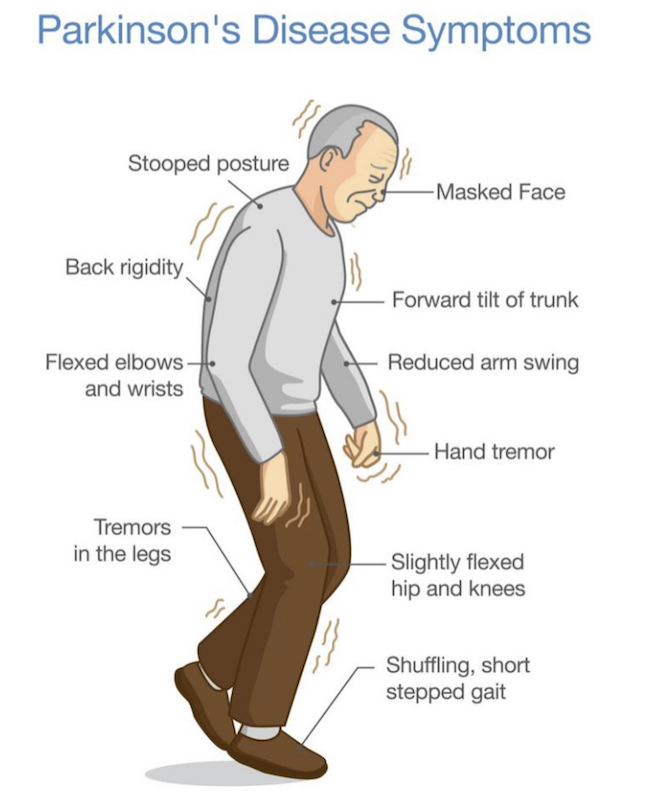
\includegraphics[width=8cm ]{slides-tex/pics/Parkinson's Disease Symptoms.png}
\caption{Parkinson's Disease Symptoms \cite{Symptoms}}
\end{figure}


\\ \hspace*{\fill} \\
Today, IMU sensors are widely used to study Parkinson's motor disease. Chapter 2 clearly describes how IMU sensors work. IMU sensors can collect motion data from the hands or feet of Parkinson's patients, and this motion data can help us analyze Parkinson's disease. However, there are many IMU sensors on the market at different prices, such as aerospace-grade sensors, which are sold at high prices and are used in military aerospace and other fields. In contrast, commercial IMU sensors are relatively inexpensive. Differences in IMU accuracy also determine price differences. Our work quantifies the loss of information when the resolution of IMU sensors is reduced. We resample the dataset collected by the original IMU sensor to create a simulated dataset collected by a low-resolution IMU sensor. After quantifying the information loss, we can infer that the IMU sensor works well at reduced resolution. First, we chose a 5-second Parkinson's time as the test dataset. We want to calculate the information loss by obtaining the predicted classification probability after classification using KNN. It is challenging to handle a super large amount of data. So we made a new step based on the mutual information between IMU data (acceleration data) and symptom score data. We want to calculate the information loss by obtaining the predicted classification probability after classification using KNN. Therefore, we obtained the information loss by simplifying the mutual information formula, as explained in Chapter 3. Chapter 5 specifies the definition of the dataset and variables we use. Chapters 6 and 7 discuss the procedures and methods for calculating the information loss based on KNN classification.

\\ \hspace*{\fill} \\












%____________________________________________________